\documentclass[]{report}
\usepackage{geometry,tikz,lipsum,amsmath,amssymb,soul,xcolor,cancel}
\usepackage[dvipsnames]{xcolor}
\tikzset{every picture/.style={line width=0.75pt}} %set default line width to 0.75pt        
\numberwithin{equation}{section}

\NewDocumentCommand{\caja}{ m O{gray!40} O{gray!10} m }{
	\begin{figure}[h]
		\centering
		\begin{tikzpicture}
			\node[anchor=text, text width=\columnwidth-1.2cm, draw, rounded corners, line width=1pt, fill=#3, inner sep=5mm] (big) {\\#4};
			\node[draw, rounded corners, line width=.5pt, fill=#2, anchor=west, xshift=5mm] (small) at (big.north west) {#1};
		\end{tikzpicture}
	\end{figure}
}
\NewDocumentCommand{\indUpDown}{ O{\Lambda} O{\mu} O{\nu} }{
	{#1}^{#2}_{\ #3}
}
\NewDocumentCommand{\indDownUp}{ O{\Lambda} O{\mu} O{\nu} }{
	{#1}_{#2}^{\ #3}
}
\newcommand{\LambdaMuNu}{\indUpDown}
\newcommand{\0}{\textcolor{gray}{0}}

\newcommand{\eff}[1]{#1_\mathrm{eff}}
\newcommand{\Ueff}{\eff{U}}

\newcommand{\rbf}{\mathbf{r}}
\newcommand{\ei}{\mathbf{e}_i}
\newcommand{\ej}{\mathbf{e}_j}
\newcommand{\lc}{\epsilon_{ijk}}
\newcommand{\gr}{\nabla}
\newcommand{\di}{\nabla\cdot}
\newcommand{\ro}{\nabla\times}
\newcommand{\la}{\nabla^2}
\newcommand{\rv}{\mathbf{r}}
\newcommand{\xv}{\mathbf{x}}
\newcommand{\yv}{\mathbf{y}}
\newcommand{\zv}{\mathbf{z}}
\newcommand{\xhat}{\hat{\xv}}
\newcommand{\yhat}{\hat{\yv}}
\newcommand{\zhat}{\hat{\zv}}
\newcommand{\rhat}{\hat{\rv}}
\newcommand{\that}{\hat{\mathbf{\theta}}}
\newcommand{\phat}{\hat{\mathbf{\varphi}}}
\newcommand{\rhhat}{\hat{\mathbf{\rho}}}
\newcommand{\nhat}{\hat{\mathbf{n}}}
\newcommand{\eo}{\epsilon_{0}}
\newcommand{\uo}{\mu_{0}}
\newcommand{\ke}{\frac{1}{4\pi\eo}}
\newcommand{\rdif}{\rv - \rv'}
\newcommand{\pd}[2]{\dfrac{\partial #1}{\partial #2}}
\newcommand{\lpd}[2]{\partial #1/\partial #2}
\newcommand{\td}[2]{\dfrac{d #1}{d #2}}
\newcommand{\ltd}[2]{d #1/d #2}
\newcommand{\n}[1]{\mathbf{#1}}

\newcommand{\GeV}{\,\text{GeV}}

%opening
\title{Ejercicios Prueba 1 Mecánica Clásica Avanzada}
\author{Simon Fonseca}

\begin{document}

\maketitle

\chapter{Formulario}

\section{Teoría de la Relatividad Especial}

\subsection{Transformaciones de Galileo y Lorentz}
\phantom{.}

Transformaciones de Galileo:
\begin{equation}
	\begin{matrix}
		x &=& x' + Vt\\
		y &=& y' \hfill\\
		z &=& z' \hfill\\
		t &=& t' \hfill
	\end{matrix}
\end{equation}

Transformaciones de Lorentz:
\begin{equation}
	\begin{matrix}
		x &=& \gamma\left({x' + Vt'}\right) \hfill\\
		y &=& y' \hfill\\
		z &=& z' \hfill\\
		ct &=& \gamma \left(ct' + \dfrac{V}{c} x'\right) \hfill
	\end{matrix}
\end{equation}
donde
\begin{equation}
	\gamma = \frac{1}{\sqrt{1 - V^2/c^2}}
\end{equation}

Intervalo (invariante de Lorentz):
\begin{equation}
	s_{12} = \sqrt{\phantom{\dfrac{\frac{}{}}{}} c^2(t_2-t_1)^2 - (x_2-x_1)^2 - (y_2-y_1)^2 - (z_2-z_1)^2}
	\label{eqn:intervalo_def}
\end{equation}

\subsection{Vectores 4-D}
Transformación de un vector 4-D:
\begin{align}
	X^\mu\rightarrow\Lambda^\mu_\nu X^\nu
\end{align}

Norma en un espacio 4-D:
\begin{equation}
	|a|^2 \equiv \sum_{\mu\nu} \eta_{\mu\nu}a^\mu a^\nu
\end{equation}

Métrica de Minkowski:
\begin{equation}
	\eta = \begin{pmatrix}
		+1 &  0 &  0 &  0\\
		 0 & -1 &  0 &  0\\
		 0 &  0 & -1 &  0\\
		 0 &  0 &  0 & -1\\
	\end{pmatrix}
\end{equation}

Usaremos la métrica para subir y bajar índices en matrices y vectores
\begin{align}
	\eta_{\mu\lambda}\LambdaMuNu &= \Lambda_{\lambda\nu}\\
	\eta_{\mu\nu}a^\nu &= a_\mu
\end{align}

La transformación de vectores y covectores se hace con diferentes matrices:
\begin{align}
	x_\mu &\rightarrow \Lambda_\mu^\nu x_\nu \\
	x^\mu &\rightarrow \Lambda^\mu_\nu x^\nu
\end{align}

Por la ortogonalidad de la métrica de Minkowski tendremos:
\begin{align}
	\eta^{\alpha\beta} \Lambda_{\alpha\mu} \Lambda_{\beta\nu} &= \eta_{\mu\nu}\\
	{\Lambda^\alpha}_\mu {\Lambda_\alpha}^\nu &= \delta^\nu_\mu
\end{align}

La generalización de boosts de Lorentz a una velocidad arbitraria $\mathbf{v}$ se puede escribir como:
\begin{align}
	\mathbf{x}' &= \mathbf{x} + \mathbf{v}\left[\frac{\mathbf{x} \cdot \mathbf{v}}{v^2} \bar{\gamma} - \gamma t\right] \\
	t' &= \gamma \left(t - \frac{\mathbf{x} \cdot \mathbf{v}}{c^2}\right)
\end{align}
donde
\begin{align}
	\gamma &= \frac{1}{\sqrt{1 - v^2/c^2}}\\
	\bar{\gamma} &= \gamma - 1
\end{align}

O, en resumen, de forma compacta y matricial:
\begin{table}[h!]
	\centering
	\begin{tabular}{ccc}
		${A^\alpha}_\mu {A_\alpha}^\nu = {\delta^\nu}_\mu, \ \ $ & $\eta_{\alpha\beta} {\Lambda^\alpha}_\mu {\Lambda_\nu}^\beta = \eta_{\mu\nu},\ \ $ & ${\Lambda_\mu}^\alpha(\mathbf{v}) = [{\Lambda^{-1}(\mathbf{v})]^\alpha}_\mu \equiv {\Lambda^\alpha}_\mu(-\mathbf{v})$
	\end{tabular}
\end{table}

donde ${\Lambda^\mu}_\nu (\mathbf{v})$ es una matriz correspondiente al boost de Lorentz:
\begin{equation}
	\begin{pmatrix}
		\gamma & -v_x\gamma & -v_y\gamma & -v_z\gamma \\
		-\dfrac{v_x\gamma}{c^2} & 1+\dfrac{\bar{\gamma}v_x^2}{v^2} & \dfrac{\bar{\gamma}v_xv_y}{v^2} & \dfrac{\bar{\gamma}v_xv_z}{v^2}\\
		-\dfrac{v_y\gamma}{c^2} & \dfrac{\bar{\gamma}v_xv_y}{v^2} & 1+\dfrac{\bar{\gamma}v_y^2}{v^2} & \dfrac{\bar{\gamma}v_yv_z}{v^2}\\
		-\dfrac{v_z\gamma}{c^2} & \dfrac{\bar{\gamma}v_xv_z}{v^2} & \dfrac{\bar{\gamma}v_yv_z}{v^2} & 1+\dfrac{\bar{\gamma}v_z^2}{v^2} \\
	\end{pmatrix}
\end{equation}

\subsection{Grupos de Lorentz}
Una transformación \(\Lambda(\theta)\) se relaciona con sus generadores \(X\) a través de
\begin{equation}
	\Lambda(\theta) = e^{\theta X}
\end{equation}

Conmutador:
\begin{equation}
	[X, Y] = XY - YX
\end{equation}

En general, tendremos la relación:
\begin{equation}
	[T_a,T_b]=f_{abc}T_c,
\end{equation}
donde \(T_a,T_b,T_c\) son vectores o elementos del grupo del álgebra, y \(f_{abc}\) es una \textbf{constante de estructura}.

Si \(\LambdaMuNu\) son las transformaciones de Lorentz posibles en 3+1 dimensiones (\(SO(1,3)\)), tendremos un grupo de Lie definido por 6 bases (\(\mathfrak{so}(1,3)\)):
\begin{itemize}
	\item 3 rotaciones espaciales (en los planos \(xy, yz, xz\)):
	\begin{equation}
		\indUpDown[J][a][bc] = -i \epsilon_{abc}
	\end{equation}
	\item 3 boosts de Lorentz (rotaciones en los planos \(xt, yt, zt\)):
	\begin{equation}
		\indUpDown[K][a\mu][\ \nu] = i(\indUpDown[\delta][\mu][a]\delta_{\nu 0} + \indUpDown[\delta][\mu][0]\delta_{\nu a})
	\end{equation}
\end{itemize}

Los generadores de los boosts y rotaciones serán entonces, respectivamente:
\begin{equation}
	\begin{matrix}
		K^x = \begin{pmatrix}
			\0 &i &\0 &\0\\
			i &\0 &\0 &\0\\
			\0 &\0 &\0 &\0\\
			\0 &\0 &\0 &\0
		\end{pmatrix} & 
		K^y = \begin{pmatrix}
			\0 &\0 &i &\0\\
			\0 &\0 &\0 &\0\\
			i &\0 &\0 &\0\\
			\0 &\0 &\0 &\0
		\end{pmatrix} &
		K^z = \begin{pmatrix}
			\0 &\0 &\0 &i\\
			\0 &\0 &\0 &\0\\
			\0 &\0 &\0 &\0\\
			i &\0 &\0 &\0
		\end{pmatrix}
	\end{matrix}
\end{equation}
\begin{equation}
	\begin{matrix}
		J^x = \begin{pmatrix}
			\0 &\0 &\0 &\0\\
			\0 &\0 &\0 &\0\\
			\0 &\0 &\0 &-i\\
			\0 &\0 &i &\0
		\end{pmatrix} & 
		J^y = \begin{pmatrix}
			\0 &\0 &\0 &\0\\
			\0 &\0 &\0 &i\\
			\0 &\0 &\0 &\0\\
			\0 &-i &\0 &\0
		\end{pmatrix} &
		J^z = \begin{pmatrix}
			\0 &\0 &\0 &\0\\
			\0 &\0 &-i &\0\\
			\0 &i &\0 &\0\\
			\0 &\0 &\0 &\0
		\end{pmatrix}
	\end{matrix}
\end{equation}

Las constantes de estructura dependerán de las diferentes combinaciones de bases, tendremos que:
\begin{equation}
	\begin{matrix}
		[K^a,K^b] = -i\epsilon_{abc}J^c,\ \ \ \ & [K^a,J^b] = i\epsilon_{abc}K^c,\ \ \ \ & [J^a,J^b] = i\epsilon_{abc}J^c
	\end{matrix}
\end{equation}

Si definimos los generadores:
\begin{equation}
	T^{(\pm)}_a = \frac{(J_a \pm iK_a)}{2}
\end{equation}
podemos definir dos subálgebras \(\left\lbrace T^{(+)}_a,T^{(-)}_a\right\rbrace\) que sí son cerradas y conmutan entre sí:
\begin{equation}
	\begin{matrix}
		[T^{(+)}_a,T^{(+)}_b] = i\epsilon_{abc}T^{(+)}_c,\ \ \ \ & [T^{(-)}_a,T^{(-)}_b] = i\epsilon_{abc}T^{(-)}_c,\ \ \ \ & [T^{(+)}_a,T^{(-)}_b] = 0
	\end{matrix}
\end{equation}
donde cada subálgebra será \(\mathfrak{so}(3)\).

Un operador Casimir (\(\mathcal{\hat{C}}\)) es aquel que conmuta con todos los generadores
\begin{equation}
	[T_a,\mathcal{\hat{C}}] = 0
\end{equation}

En el caso del álgebra de Lorentz tenemos dos Casimires:
\begin{equation}
	\mathcal{\hat{C}}_{\pm} = \sum_{a}(T_a^{\pm})^2 = \frac{\mathbf{J}^2-\mathbf{K}^2}{4} \pm i\frac{\mathbf{J}\cdot\mathbf{K}}{2}
\end{equation}

En el caso del espacio de representación de Minkowski, tendremos que ambos Casimires serán:
\begin{equation}
	\mathcal{\hat{C}}_{\pm} = \frac{3}{4}\mathbb{I}
\end{equation}

\subsection{Formulación covariante}

El símbolo de Levi-Civita en 3 dimensiones  se debe cambiar por su versión en 4 dimensiones (pero funciona igual).
\begin{equation}
	\epsilon_{abc} \rightarrow \epsilon_{\mu\nu\alpha\beta}
\end{equation}

Los vectores:
\begin{equation}
	\vec{a} \rightarrow a^\mu, a_\mu = \eta_{\mu\nu}a^\nu
\end{equation}

El producto escalar:
\begin{equation}
	\vec{a}\cdot\vec{b} \rightarrow a_\mu b^\mu \equiv \eta_{\mu\nu}a^\mu b^\nu
\end{equation}

En vez de productos cruz (solo definido en 3-D):
\begin{equation*}
	\vec{A}\times\vec{B} = (A_j B_k - A_k B_j)\hat{i} + (A_k B_i - A_i B_k)\hat{j} + (A_i B_j - A_j B_i)\hat{k}
\end{equation*}
tendremos un \textit{bivector}, un tensor antisimétrico de rango 2 :
\begin{equation}
	A\wedge B = \frac{1}{2}(A^\mu B^\nu - A^\nu B^\mu)
\end{equation}

El gradiente:
\begin{equation}
	\vec{\nabla} f \rightarrow \partial_\mu f
\end{equation}

La divergencia:
\begin{equation}
	\nabla\cdot\vec{a} \equiv \partial_k a^k \rightarrow \partial_\mu f^\mu \equiv \eta^{\mu\nu}\partial_\mu f_\nu
\end{equation}

El rotacional:
\begin{equation}
	\vec{\nabla}\times\vec{a} \rightarrow \partial_\mu a_\nu - \partial_\nu a_\mu
\end{equation}

El laplaciano:
\begin{equation}
	\Delta \equiv \nabla^2 \equiv \partial_k^2 \rightarrow \square \equiv \partial_\mu\partial^\mu = \frac{\partial_t^2}{c^2} - \Delta
\end{equation}

En vez de un elemento de superficie:
\begin{align*}
	d\vec{S} = d\vec{a} \times d\vec{b} &= (da_j db_k - da_k db_j)\hat{i} + (da_k db_i - da_i db_k)\hat{j} + (da_i db_j - da_j db_i)\hat{k}\\
	&= \hat{n}\left|dS\right| 
\end{align*}
tendremos el elemento de superficie (una 2-forma, bivector):
\begin{equation}
	dS^{\mu\nu} = da^\mu db^\nu - db^\mu da^\nu
\end{equation}

\subsubsection{4-velocidad}
\phantom{.}

El tiempo propio medido en el marco de referencia de la partícula:
\begin{equation}
	d\tau = \sqrt{1-v^2/c^2}dt
\end{equation}

La 4-velocidad:
\begin{align}
	u^\mu \equiv \frac{dx^mu}{d\tau} &= \left(\dfrac{c}{\sqrt{1 - v^2/c^2}}, \dfrac{\vec{v}}{\sqrt{1 - v^2/c^2}} \right) \\
	u^\mu &= \left(\gamma c, \gamma\vec{v} \right)
\end{align}

La norma del vector 4-velocidad cumple con:
\begin{equation}
	u_\mu u^\mu \equiv \eta_{\mu\nu}u^\mu u^\nu = c^2
\end{equation}

Si conocemos todas las componentes de la 4-velocidad, podemos recuperar la velocidad normal sin conocer directamente el valor \(\gamma\) a través de:
\begin{equation}
	v^i = c\frac{u^i}{u^0}
\end{equation}

\subsubsection{4-momento}
\phantom{.}

El 4-momento:
\begin{equation}
	p^\mu \equiv mu^\mu = \left(\dfrac{mc}{\sqrt{1 - v^2/c^2}}, \dfrac{m\vec{v}}{\sqrt{1 - v^2/c^2}} \right) 
\end{equation}

De donde identificamos los componentes:
\begin{equation}
	\begin{matrix}
		p^\mu  = \left(\dfrac{E}{c}, \vec{p}\right), & E = \gamma mc^2, & \vec{p} = \gamma m\vec{v}
	\end{matrix}
\end{equation}

De aquí sale la relación de energía momento
\begin{align}
	E^2 - \vec{p}^{\ 2}c^2 &= m^2c^4 \label{eqn:relacion_energia_momento}\\
	\Rightarrow E &= \sqrt{m^2c^4 + \sum p_i^2c^2}
\end{align}

Por construcción, los componentes del 4-vector \(p^\mu\) transforman como coordenadas \(x^\mu\) o 4-velocidad \(u^\mu\):
\begin{equation}
	p'^\mu = \LambdaMuNu p^\nu
\end{equation}

Para un sistema de \(n\) partículas usaremos la notación:
\begin{equation}
	P^\mu = \sum_i^n p^\mu_i
\end{equation}

\subsubsection{4-fuerza}
\phantom{.}

La 4-fuerza:
\begin{equation}
	g^\mu \equiv \frac{dp^\mu}{d\tau} = \left(\dfrac{\vec{f}\cdot\vec{v}}{c\sqrt{1 - v^2/c^2}}, \dfrac{\vec{f}}{\sqrt{1 - v^2/c^2}} \right) 
\end{equation}
donde \(\vec{f}\) es la 3-fuerza \(\vec{f}=d\vec{p}/dt\).

Además se cumplirá que:
\begin{equation}
	u^\mu g_\mu = 0
\end{equation}

\subsection{Colisiones}
La masa invariante del sistema debe mantenerse constante
\begin{equation}
	P^\mu P_\mu = M^2c^2
\end{equation}

Para una colisión \(1+2\rightarrow 3+4\) tenemos 16 variables para definir todo el sistema, ya que tendremos 4 partículas con 4 componentes de 4-momento (energía, \(p_x,p_y,p_z\)). Sin embargo, podemos definir una serie de ecuaciones que restringirán al sistema y reducirán el número de partículas:
\begin{itemize}
	\item De la ecuación \ref{eqn:relacion_energia_momento} tenemos la condición de masa \textit{on shell} que nos da una ecuación para cada partícula (\textbf{4 en total}):
	\begin{equation*}
		E_i^2 - \vec{p}_i^{\ 2}c^2 = m_i^2c^4
	\end{equation*}
	\item De la conservación de 4-momento sacamos una ecuación por componente (\textbf{4 en total}):
	\begin{equation*}
		P^\mu_{\text{inicial}} = P^\mu_{\text{final}}
	\end{equation*}
	\item Podemos exigir que una de las partículas se mantenga en reposo al momento de la colisión, lo que nos daría expresiones para anular los componentes espaciales de su momento (\textbf{3 en total}).
	\begin{equation*}
		\vec{p}_2 = \vec{0}
	\end{equation*}
	\item También podemos hacer una rotación espacial para hacer coincidir la dirección del momento con el eje \(z\), dándonos 2 expresiones para anular las otras componentes del momento espacial (\textbf{2 en total}):
	\begin{equation*}
		p_{1x} = 0,\ \ \ p_{1y} = 0
	\end{equation*}
	\item Además podemos hacer una rotación espacial alrededor del eje \(z\), tal que el plano formado por las partículas post-colisión coincida con el plano \(xz\) (\textbf{1 en total}):
	\begin{equation*}
		p_{3y} = 0
	\end{equation*}
\end{itemize}

Las invariantes de Mandelstam describen una colisión elástica y son invariantes ante una transformación de Lorentz:
\begin{align}
	s &\equiv (p^\mu_{1i} + p^\mu_{2i})^2 = (p^\mu_{1f} + p^\mu_{2f})^2\\
	t &\equiv (p^\mu_{1f} - p^\mu_{1i})^2 = (p^\mu_{2f} - p^\mu_{2i})^2\\
	u &\equiv (p^\mu_{1f} - p^\mu_{2i})^2 = (p^\mu_{2f} - p^\mu_{1i})^2
\end{align}

En una colisión \(1 + 2 \rightarrow 3 + 4\) tendremos:
\begin{equation}
	s+t+u = m_1^2 + m_2^2 + m_3^2 + m_4^2
\end{equation}




\section{Formulación Lagrangiana}

\subsection{Acción y lagrangiano}

La acción:
\begin{equation}
	 S = \int_{t_1}^{t_2} L(q_i,\dot{q}_k,t) dt
\end{equation}

La acción y el lagrangiano están definidos para todo el sistema, no para partículas individuales.

La formulación lagrangiana es equivalente a la formulación newtoniana para fuerzas conservativas. Si tomamos:
\begin{equation}
	L = T - U = \sum_{a=1}^{3n}\frac{m \dot{q}_a^2}{2} - U(q_1,\ldots,q_{3n})
\end{equation}
entonces la Segunda Ley de Newton \(m\ddot{\mathbf{q}} = -\nabla U(\mathbf{b})\) es equivalente a las \textbf{ecuaciones de Euler-Lagrange}:
\begin{align}
	\frac{\partial L}{\partial q_a} - &\frac{d}{dt}\left(\frac{\partial L}{\partial \dot{q}_a}\right) = 0,\label{E-L_ecs}\\
	p_a \equiv \frac{\partial L}{\partial\dot{q}_a},&\ \ \ \ \ \ a = 1,\ldots,N\nonumber
\end{align}
para un sistema con \(N\) coordenadas independientes.

Multiplicación por una constante arbitraria no cambia las ecuaciones de movimiento:
\begin{equation}
	L(q,\dot{q},t) \rightarrow \textcolor{red}{\lambda} L(q_i,\dot{q}_k,t)
\end{equation}

Sumar una derivada completa (\(d/dt\)) de una función arbitraria \(f(q,t)\) tampoco cambia las ecuaciones de movimiento:
\begin{equation}
	L(q,\dot{q},t) \rightarrow L(q_i,\dot{q}_k,t) + \textcolor{red}{\frac{d}{dt}f(q,t)}
\end{equation}

\subsection{Coordenadas curvilíneas}
Tomando una transformación de variables arbitraria:
\begin{equation*}
	q_a = q_a(r_1, r_2, r_3),\ \ \ \ \ a=1,2,3
\end{equation*}
Tendremos que el lagrangiano vendrá dado por:
\begin{equation}
	L = \sum_{a,b=1}^{3} \frac{\mu_{ab}(r)\dot{r}_a \dot{r}_a}{2} - U(r_a)
\end{equation}
donde
\begin{equation}
	\mu_{ab}(r) = m \sum_{k=1}^{3}\dfrac{\partial q_k}{\partial r_a}\dfrac{\partial q_k}{\partial r_b} = m g_{ab}
\end{equation}
donde \(g_{ab}\) es el tensor métrico. En el caso de coordenadas ortogonales (esféricas, cilíndricas, elípticas, parabólicas), tendremos:
\begin{equation}
	g_{ab} = h_a^2\delta_{ab}
\end{equation}
donde \(h_a\) son los \textbf{coeficientes de Lamé}.

Las ecuaciones de Euler-Lagrange son \textbf{covariantes ante transformaciones de variables}.

\subsection{Formalismo lagrangiano}
Para cualquier conjunto de variables \({q_a}\) que caracterizan las posiciones de los cuerpos del sistema, tendremos el \textbf{momento generalizado}:
\begin{equation}
	p_k \equiv \frac{\partial L}{\partial \dot{q}_k}
\end{equation}
y la \textbf{fuerza generalizada}:
\begin{equation}
	f_k \equiv \frac{\partial L}{\partial q_k}
\end{equation}
Y obtenemos una ecuación similar a la Segunda Ley de Newton
\begin{equation}
	\dot{p}_k = f_k = \frac{\partial L}{\partial q_k}
\end{equation}
Si además consideramos la velocidad:
\begin{equation}
	\mathbf{v} \equiv \frac{d \mathbf{r}}{dt} = \sum h_a \dot{r}_a \mathbf{e}_a
\end{equation}
tendremos la aceleración:
\begin{equation}
	\mathbf{a} \equiv \frac{d \mathbf{v}}{dt} = \sum h_a\ddot{r}_a\mathbf{e}_a + \sum \frac{\partial h_a}{\partial r_b}\dot{r}_a\dot{r}_b\mathbf{e}_a + \sum h_a\dot{r}_a\frac{d\mathbf{e}_a}{dt}
\end{equation}
De aquí, el término \(\dfrac{d\mathbf{e}_a}{dt}\) puede ser escrito según los coeficientes de Lamé:
\begin{equation}
	\frac{d\mathbf{e}_a}{dt} = \sum_{b}\frac{d\mathbf{e}_a}{dr_b}\dot{r}_b = \sum_{b,c} \Gamma^{c}_{ab} \mathbf{e}_a \dot{r}_b
\end{equation}
donde \(\Gamma^{c}_{ab}\) son los \textbf{símbolos de Christoffel}
\begin{equation}
	\Gamma^{c}_{ab} = \left(\mathbf{e}^c \cdot \frac{d\mathbf{e}_a}{dr_b}\right)
\end{equation}
que pueden ser escritos en función de la métrica
\begin{equation}
	\Gamma^{c}_{ab} = \frac{1}{2} g^{cd} \left(\frac{\partial g_{ad}}{\partial r^b} + \frac{\partial g_{bd}}{\partial r^a} - \frac{\partial g_{ab}}{\partial r^d}\right)
\end{equation}
y, en el caso de coordenadas ortogonales (\(g_{ab} = h_a^2\delta_{ab}\)), podremos reescribirlo dependiendo de \(h_a\):
\begin{equation}
	\Gamma^{c}_{ab} = \left(\delta_{ac}\frac{\partial \ln h_{a}}{\partial r^b} + \delta_{bc}\frac{\partial \ln h_{c}}{\partial r^a} - \frac{\delta_{ab}}{2 h_c^2}\frac{\partial h_{a}^2}{\partial r^c}\right)
\end{equation}

\subsection{Integrales de movimiento y Teorema de Noether}
Si el lagrangiano \(L\) de un sistema con \(n\) grados de libertad es invariante con respecto a
\begin{align*}
	q_a(t) &\rightarrow q_a(t) + \epsilon\gamma_a(t)\\
	\dot{q}_a(t) &\rightarrow \dot{q}_a(t) + \epsilon\dot{\gamma}_a(t)\\
	t &\rightarrow t
\end{align*}
donde \(\epsilon = \mathrm{const}\) es un parámetro continuo. Entonces la cantidad
\begin{equation}
	Q = \sum_{a}\frac{\partial L}{\partial \dot{q}_a}\gamma_a
\end{equation}
es conservada.

\subsection{Movimiento en campo central}
El potencial efectivo:
\begin{equation}
	\Ueff(r) = U(r) + \frac{M^2}{2 m r^2}
\end{equation}

Tendremos entonces un movimiento efectivo en una dimensión (radial). Tomando
\begin{align}
	\td{r}{t} &= \sqrt{\frac{2}{m} \left[E - U_\mathrm{eff}(r)\right]}\\
	M &\equiv m r^2 \dot{\varphi} = \mathrm{const.}
\end{align}
encontramos la forma de la trayectoria \(r = r(\varphi)\) como
\begin{equation}
	\varphi - \varphi_0 = \int_{r_0}^{r} dr \frac{M}{m r^2 \sqrt{\frac{2}{m} \left(E - U_\mathrm{eff}(r)\right)}}
\end{equation}

En el caso del potencial de Coulomb (\(U(r) \propto -1/r\)), la trayectoria vendrá dada por
\begin{equation}
	\frac{p}{r} = 1 + e \cos \phi
\end{equation}
donde \(p\) es el \textit{semilatus rectum}
\begin{equation}
	p = \frac{M^2}{m\alpha}
\end{equation}
y la excentricidad de la órbita
\begin{equation}
	e = \sqrt{1 + \frac{2 E M^2}{m \alpha^2}}
\end{equation}

Para un potencial general, todas las órbitas con un momento angular \(\mathbf{M}\) y energía \(E = \Ueff(r_\mathrm{min})\), donde \(r_\mathrm{min}\) es la solución de
\begin{equation}
	-\frac{M^2}{m r_\mathrm{min}^3} + U'(r_\mathrm{min}) = 0 \label{EDO_orb_cerrada}
\end{equation}
son \textbf{cerradas}.

\chapter{Ejercicios de relatividad}
\section{Ejercicio 1}
The accelerator SuperKEKB collides electrons (\(e^{-}\)) of energy \(E_{1} = 7\) GeV with positrons (\(e^{+}\)) of energy \(E_{2} = 4\) GeV. Before the collision, both particles move in opposite directions along the axis \(z\) (collision axis in what follows). After the collision, two oppositely charged \(B\)-mesons (\(B^{+}\) and \(B^{-}\)) are produced via the process \(e^{+}\, e^{-} \rightarrow B^{+}\, B^{-}\), and one of the \(B\)-mesons emerges at angle \(\alpha_{1}\) with respect to the collision axis. The rest frame masses of both \(B\)-mesons are equal to each other, whereas masses of electron and positron are negligibly small.
\begin{enumerate}
	\item[a)] Find the energies of the produced \(B\)-mesons \(\mathcal{E}_{1}, \mathcal{E}_{2}\) in the laboratory frame and their relative velocity \(v_{\mathrm{rel}}\). Your result should be expressed as a function of the angle \(\alpha\) and energies of the incoming particles.
	\item[b)] Assume that You can vary the energy of electrons \(E_{1}\), whereas the energy of positrons \(E_{2}\) remains fixed. Find the minimal electron energy \(E_{1, \mathrm{min}}\) required for this process.
	\item[c)] Write out explicit expressions for the Mandelstam variables \(s, t, u\) in terms of energies \(E_{1}, E_{2}\) and the angle \(\alpha\) in the lab frame.
\end{enumerate}
\begin{figure}[h!]
	\centering
	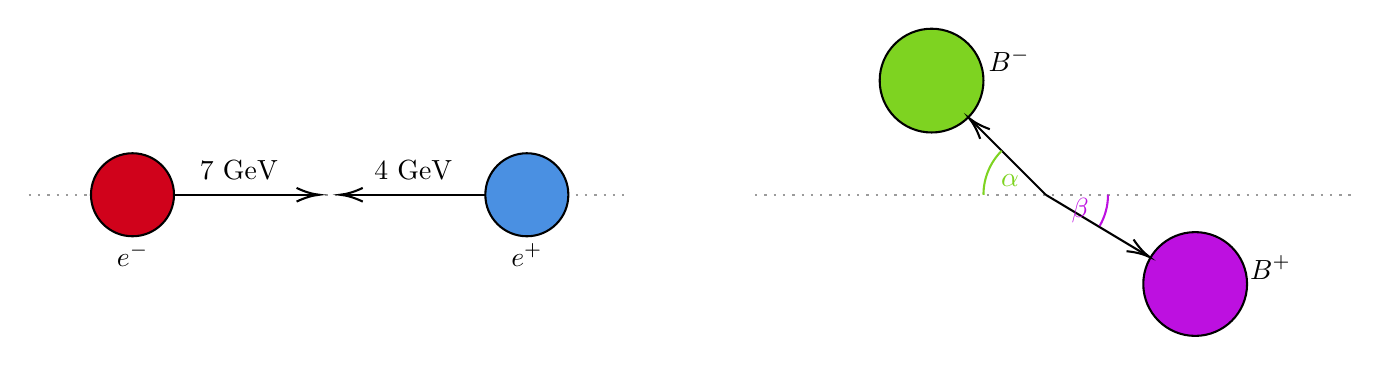
\begin{tikzpicture}[x=0.75pt,y=0.75pt,yscale=-1,xscale=1]
		%uncomment if require: \path (0,300); %set diagram left start at 0, and has height of 300
		
		%Straight Lines [id:da2666196383049946] 
		\draw [color={rgb, 255:red, 155; green, 155; blue, 155 }  ,draw opacity=1 ] [dash pattern={on 0.84pt off 2.51pt}]  (10,90) -- (300,90) ;
		%Shape: Circle [id:dp5941497912321755] 
		\draw  [fill={rgb, 255:red, 208; green, 2; blue, 27 }  ,fill opacity=1 ] (40,90) .. controls (40,78.95) and (48.95,70) .. (60,70) .. controls (71.05,70) and (80,78.95) .. (80,90) .. controls (80,101.05) and (71.05,110) .. (60,110) .. controls (48.95,110) and (40,101.05) .. (40,90) -- cycle ;
		%Shape: Circle [id:dp5300941970691377] 
		\draw  [fill={rgb, 255:red, 74; green, 144; blue, 226 }  ,fill opacity=1 ] (230,90) .. controls (230,78.95) and (238.95,70) .. (250,70) .. controls (261.05,70) and (270,78.95) .. (270,90) .. controls (270,101.05) and (261.05,110) .. (250,110) .. controls (238.95,110) and (230,101.05) .. (230,90) -- cycle ;
		%Straight Lines [id:da791965915355674] 
		\draw    (80,90) -- (148,90) ;
		\draw [shift={(150,90)}, rotate = 180] [color={rgb, 255:red, 0; green, 0; blue, 0 }  ][line width=0.75]    (10.93,-3.29) .. controls (6.95,-1.4) and (3.31,-0.3) .. (0,0) .. controls (3.31,0.3) and (6.95,1.4) .. (10.93,3.29)   ;
		%Straight Lines [id:da5138005195075709] 
		\draw    (230,90) -- (162,90) ;
		\draw [shift={(160,90)}, rotate = 360] [color={rgb, 255:red, 0; green, 0; blue, 0 }  ][line width=0.75]    (10.93,-3.29) .. controls (6.95,-1.4) and (3.31,-0.3) .. (0,0) .. controls (3.31,0.3) and (6.95,1.4) .. (10.93,3.29)   ;
		%Straight Lines [id:da4344549993609035] 
		\draw [color={rgb, 255:red, 155; green, 155; blue, 155 }  ,draw opacity=1 ] [dash pattern={on 0.84pt off 2.51pt}]  (360,90) -- (650,90) ;
		%Shape: Circle [id:dp5014291513295692] 
		\draw  [fill={rgb, 255:red, 126; green, 211; blue, 33 }  ,fill opacity=1 ] (420,35) .. controls (420,21.19) and (431.19,10) .. (445,10) .. controls (458.81,10) and (470,21.19) .. (470,35) .. controls (470,48.81) and (458.81,60) .. (445,60) .. controls (431.19,60) and (420,48.81) .. (420,35) -- cycle ;
		%Shape: Circle [id:dp2010294594289822] 
		\draw  [fill={rgb, 255:red, 189; green, 16; blue, 224 }  ,fill opacity=1 ] (547,133) .. controls (547,119.19) and (558.19,108) .. (572,108) .. controls (585.81,108) and (597,119.19) .. (597,133) .. controls (597,146.81) and (585.81,158) .. (572,158) .. controls (558.19,158) and (547,146.81) .. (547,133) -- cycle ;
		%Straight Lines [id:da9297103902850272] 
		\draw    (500,90) -- (464.41,54.41) ;
		\draw [shift={(463,53)}, rotate = 45] [color={rgb, 255:red, 0; green, 0; blue, 0 }  ][line width=0.75]    (10.93,-3.29) .. controls (6.95,-1.4) and (3.31,-0.3) .. (0,0) .. controls (3.31,0.3) and (6.95,1.4) .. (10.93,3.29)   ;
		%Straight Lines [id:da9786927386703091] 
		\draw    (500,90) -- (548.29,118.97) ;
		\draw [shift={(550,120)}, rotate = 210.96] [color={rgb, 255:red, 0; green, 0; blue, 0 }  ][line width=0.75]    (10.93,-3.29) .. controls (6.95,-1.4) and (3.31,-0.3) .. (0,0) .. controls (3.31,0.3) and (6.95,1.4) .. (10.93,3.29)   ;
		%Shape: Arc [id:dp2642691597839596] 
		\draw  [draw opacity=0] (470,90) .. controls (470,81.72) and (473.36,74.22) .. (478.79,68.79) -- (500,90) -- cycle ; \draw  [color={rgb, 255:red, 126; green, 211; blue, 33 }  ,draw opacity=1 ] (470,90) .. controls (470,81.72) and (473.36,74.22) .. (478.79,68.79) ;  
		%Shape: Arc [id:dp1349982239947891] 
		\draw  [draw opacity=0] (530,90) .. controls (530,90) and (530,90) .. (530,90) .. controls (530,90) and (530,90) .. (530,90) .. controls (530,95.47) and (528.54,100.59) .. (525.99,105) -- (500,90) -- cycle ; \draw  [color={rgb, 255:red, 189; green, 16; blue, 224 }  ,draw opacity=1 ] (530,90) .. controls (530,90) and (530,90) .. (530,90) .. controls (530,90) and (530,90) .. (530,90) .. controls (530,95.47) and (528.54,100.59) .. (525.99,105) ;  
		
		% Text Node
		\draw (51,112) node [anchor=north west][inner sep=0.75pt]   [align=left] {$\displaystyle e^{-}$};
		% Text Node
		\draw (241,112) node [anchor=north west][inner sep=0.75pt]   [align=left] {$\displaystyle e^{+}$};
		% Text Node
		\draw (91,72) node [anchor=north west][inner sep=0.75pt]   [align=left] {7 GeV};
		% Text Node
		\draw (175,72) node [anchor=north west][inner sep=0.75pt]   [align=left] {4 GeV};
		% Text Node
		\draw (477,79) node [anchor=north west][inner sep=0.75pt]  [color={rgb, 255:red, 126; green, 211; blue, 33 }  ,opacity=1 ] [align=left] {$\displaystyle \alpha $};
		% Text Node
		\draw (511,90) node [anchor=north west][inner sep=0.75pt]  [color={rgb, 255:red, 189; green, 16; blue, 224 }  ,opacity=1 ] [align=left] {$\displaystyle \beta $};
		% Text Node
		\draw (471,18) node [anchor=north west][inner sep=0.75pt]   [align=left] {$\displaystyle B^{-}$};
		% Text Node
		\draw (597,118) node [anchor=north west][inner sep=0.75pt]   [align=left] {$\displaystyle B^{+}$};
	\end{tikzpicture}
\end{figure}

\begin{enumerate}
	\item[a)] Tomamos \(c = 1\). Asumiendo que \(YZ\) es el plano de scattering, tenemos
	\begin{equation}
		\begin{pmatrix}
			p^{\mu}_{e^{-}}\\
			p^{\mu}_{e^{+}}\\
			p^{\mu}_{B^{-}}\\
			p^{\mu}_{B^{+}}
		\end{pmatrix} = \begin{pmatrix}
			E_{1} 			& \0 & \0 								& |\vec{p}_{e^{-}}|\\
			E_{2} 			& \0 & \0 								& -|\vec{p}_{e^{+}}|\\
			\mathcal{E}_{1} & \0 & \hfill|\vec{p}_{B^{-}}|\sin\alpha	& -|\vec{p}_{B^{-}}|\cos\alpha\\
			\mathcal{E}_{2} & \0 & -|\vec{p}_{B^{+}}|\sin\beta 		& \hfill|\vec{p}_{B^{+}}|\cos\beta
		\end{pmatrix}
	\end{equation}
	
	Si realizamos un boost en la dirección \(z\) al marco CM, tendremos
	\begin{equation}
		\LambdaMuNu(v) = \begin{pmatrix}
			\gamma & \0 & \0 & -\gamma v\\
			\0 & 1 & \0 & \0\\
			\0 & \0 & 1 & \0\\
			-\gamma v & \0 & \0 & \gamma
		\end{pmatrix}
	\end{equation}
	donde \(v = (|\vec{p}_{e^{-}}| - |\vec{p}_{e^{+}}|)/(E_{1} + E_{2})\). Tendremos entonces
	\begin{equation}
		\begin{pmatrix}
			p'^{\mu}_{e^{-}}\\
			p'^{\mu}_{e^{+}}\\
			p'^{\mu}_{B^{-}}\\
			p'^{\mu}_{B^{+}}
		\end{pmatrix} = \begin{pmatrix}
			E' 			 & \0 & \0 								& |\vec{p'}_{e}|\\
			E' 			 & \0 & \0 								& -|\vec{p'}_{e}|\\
			\mathcal{E}' & \0 & \hfill|\vec{p'}_{B}|\sin\psi	& -|\vec{p'}_{B}|\cos\psi\\
			\mathcal{E}' & \0 & -|\vec{p'}_{B}|\sin\psi 		& \hfill|\vec{p'}_{B}|\cos\psi
		\end{pmatrix}
	\end{equation}
	donde
	\begin{equation}
		E' = \frac{E_{1} (E_{1}+E_{2})+|\vec{p}_{e^{-}}| (|\vec{p}_{e^{+}}|-|\vec{p}_{e^{-}}|)}{(E_{1}+E_{2}) \sqrt{1-\frac{(|\vec{p}_{e^{-}}|-|\vec{p}_{e^{+}}|)^2}{(E_{1}+E_{2})^2}}}
	\end{equation}
	pero, en el caso de los electrones con masa \(m_{e} \approx 0\)
	\begin{equation*}
		E = \sqrt{m^2 + \vec{p}^2} \approx |\vec{p}|
	\end{equation*}
	por lo que
	\begin{equation}
		E' \approx \sqrt{E_{1} E_{2}}
	\end{equation}
	
	De la conservación de energía-momento:
	\begin{align}
		\mathcal{E}' &= E'
		%		|\vec{p'}_{B^{-}}|\sin\alpha' &= |\vec{p'}_{B^{+}}|\sin\beta'\\
		%		E'_{1} &= -|\vec{p'}_{B^{-}}|\cos\alpha' + |\vec{p'}_{B^{+}}|\cos\beta'
	\end{align}
	Basándonos en la condición  de masa \textit{on-shell} y que \(m_{e} \approx 0\):
	\begin{align}
		E' & \approx |\vec{p'}_{e}|\label{onShell_1}\\
%		E'_{2} & \approx |\vec{p'}_{e^{-}}|\label{onShell_2}\\
%		\mathcal{E}'_{1} &= \sqrt{m_{B}^2 + |\vec{p'}_{B^{-}}|^{2}}\label{onShell_3}\\
|\vec{p'}_{B}| &= \sqrt{\mathcal{E}'^{2} - m_{B}^2}\label{onShellInv_4}
	\end{align}
	
	Por lo que
	\begin{equation}
		\begin{pmatrix}
			p'^{\mu}_{e^{-}}\\
			p'^{\mu}_{e^{+}}\\
			p'^{\mu}_{B^{-}}\\
			p'^{\mu}_{B^{+}}
		\end{pmatrix} = \begin{pmatrix}
			\sqrt{E_{1} E_{2}} & \0 & \0 								&  \sqrt{E_{1} E_{2}}\\
			\sqrt{E_{1} E_{2}} & \0 & \0 								& -\sqrt{E_{1} E_{2}}\\
			\sqrt{E_{1} E_{2}} & \0 & \hfill\sqrt{E_{1} E_{2} - m_{B}^2}\sin\psi	& -\sqrt{E_{1} E_{2} - m_{B}^2}\cos\psi\\
			\sqrt{E_{1} E_{2}} & \0 & -\sqrt{E_{1} E_{2} - m_{B}^2}\sin\psi 		& \hfill\sqrt{E_{1} E_{2} - m_{B}^2}\cos\psi
		\end{pmatrix}
	\end{equation}
	Y, volviendo al marco del laboratorio con \(\LambdaMuNu(-v)\),
	\begin{equation}
		\begin{pmatrix}
			p^{\mu}_{e^{-}}\\
			p^{\mu}_{e^{+}}\\
			p^{\mu}_{B^{-}}\\
			p^{\mu}_{B^{+}}
		\end{pmatrix} \approx \begin{pmatrix}
			E_{1} & \0 & \0 								&  E_{1}\\
			E_{2} & \0 & \0 								& -E_{2}\\
			\frac{1}{2}\left(E_{1} + E_{2} + E_{B}^{-}\right) & \0 & ~~\sqrt{E_{1} E_{2} - m_{B}^2}\sin\psi	& \frac{1}{2}\left(E_{1} - E_{2} - E_{B}^{+}\right)\\
			\frac{1}{2}\left(E_{1} + E_{2} - E_{B}^{-}\right) & \0 & -\sqrt{E_{1} E_{2} - m_{B}^2}\sin\psi & \frac{1}{2}\left(E_{1} - E_{2} + E_{B}^{+}\right)
		\end{pmatrix}
	\end{equation}
	donde
	\begin{equation}
		E_{B}^{\pm} = \frac{(E_{2}\pm E_{1})\sqrt{E_{1} E_{2}-m_{B}^2}}{\sqrt{E_{1} E_{2}}}\cos\psi 
	\end{equation}
	Explícitamente,
	\begin{align}
		\mathcal{E}_{1} = \frac{1}{2} \left(E_{1} + E_{2} + \frac{(E_{2} - E_{1})\sqrt{E_{1} E_{2}-m_{B}^2}}{\sqrt{E_{1} E_{2}}}\cos\psi\right)
	\end{align}
	La relación entre \(\psi\) y $\alpha$ es complicada, mira en Mathematica.
%	Además
%	\begin{equation}
%		\left(p^{\mu}_{B^{-}}\right)^{2} = \left(p^{\mu}_{e^{-}} + p^{\mu}_{e^{+}} - p^{\mu}_{B^{+}} \right)^{2}
%	\end{equation}
%	pero \(\left(p^{\mu}\right)^{2} = m^2\), por lo que
%	\begin{align*}
%		m_{B^{-}}^{2} &= m_{e^{-}}^{2} + m_{e^{+}}^{2} + m_{B^{+}}^{2} + \textcolor{red}{\left(p'_{e^{-}}\right)^{\lambda}\left(p'_{e^{+}}\right)_{\lambda}} - \textcolor{blue}{\left(p'_{e^{-}}\right)^{\alpha}\left(p'_{B^{+}}\right)_{\alpha}} - \textcolor{purple}{\left(p'_{e^{+}}\right)^{\beta}\left(p'_{B^{+}}\right)_{\beta}}\\
%		0 &= \textcolor{red}{\left(E'^{2} + |\vec{p'}_{e}|^2\right)} - \textcolor{blue}{\left(E'^{2} - |\vec{p'}_{e}||\vec{p'}_{B}|\cos\psi\right)} - \textcolor{purple}{\left(E'_{2}\mathcal{E}'_{2} + |\vec{p'}_{e^{+}}||\vec{p'}_{B^{+}}|\cos\beta'\right)}
%	\end{align*}
%	Reemplazando ecs. \ref{onShell_1} y \ref{onShell_2}
%	\begin{align}
%		0 &\approx \textcolor{blue}{- E'_{1}\mathcal{E}'_{2} + E'_{1}|\vec{p'}_{B^{+}}|\cos\beta'}\nonumber\\
%		\Rightarrow \mathcal{E}'_{2} &\approx |\vec{p'}_{B^{+}}|\cos\beta'\\
%		\intertext{Siguiendo el mismo procedimiento para \(|\vec{p'}_{B^{-}}|\cos\alpha'\)}
%		\Rightarrow \mathcal{E}'_{1} &\approx -|\vec{p'}_{B^{-}}|\cos\alpha'
%	\end{align}
%	Introduciendo estos resultados en las ecs. \ref{onShell_3} y \ref{onShell_4}:
%	\begin{align}
%		|\vec{p'}_{B^{-}}|^2\cos^2\alpha' &= m_{B}^2 + |\vec{p'}_{B^{-}}|^{2}\nonumber\\
%		|\vec{p'}_{B^{-}}|^2\left(\cos^2\alpha' - 1\right) &= m_{B}^2\nonumber\\
%		\Rightarrow -|\vec{p'}_{B^{-}}| \sin\alpha' &= m_{B}
%	\end{align}
%	\begin{align}
%		|\vec{p'}_{B^{+}}|^2\cos^2\beta' &= m_{B}^2 + |\vec{p'}_{B^{+}}|^{2}\nonumber\\
%		|\vec{p'}_{B^{+}}|^2\left(\cos^2\beta' - 1\right) &= m_{B}^2\nonumber\\
%		\Rightarrow -|\vec{p'}_{B^{+}}|\sin\beta' &= m_{B}
%	\end{align}
%	Sumando ambos términos
%	\begin{equation}
%		\Rightarrow |\vec{p}_{B^{+}}|\cos\beta + |\vec{p}_{B^{-}}|\cos\alpha = - \frac{\left(E_{1} + E_{2}\right) \left(\mathcal{E}_{1} - \mathcal{E}_{2}\right)}{E_{1} - E_{2}}
%	\end{equation}
%	Luego
%	\begin{align}
%		|\vec{p}_{B^{+}}|^{2}\sin^{2}\beta &= |\vec{p}_{B^{-}}|^{2}\sin^{2}\alpha\\
%		|\vec{p}_{B^{+}}|^{2}\cos^{2}\beta &= E^{2}_{\mathrm{T}} + |\vec{p}_{B^{-}}|^{2}\cos^{2}\alpha + 2 E_{\mathrm{T}}|\vec{p}_{B^{-}}|\cos\alpha\\
%		\Rightarrow |\vec{p}_{B^{+}}|^{2}  &= |\vec{p}_{B^{-}}|^{2} + E^{2}_{\mathrm{T}} + 2 E_{\mathrm{T}}|\vec{p}_{B^{-}}|\cos\alpha
%	\end{align}
%	pero 
	
\end{enumerate}

\chapter{Ejercicios de lagrangianos}





























\end{document}